\begin{tikzpicture}[every node/.style={inner sep=0pt}]
\foreach \coord/\name in {{(0,0)}/first,{(2.7,0.3)}/second,{(5.4,0)}/third} {
	\node (\name-cpu) at \coord {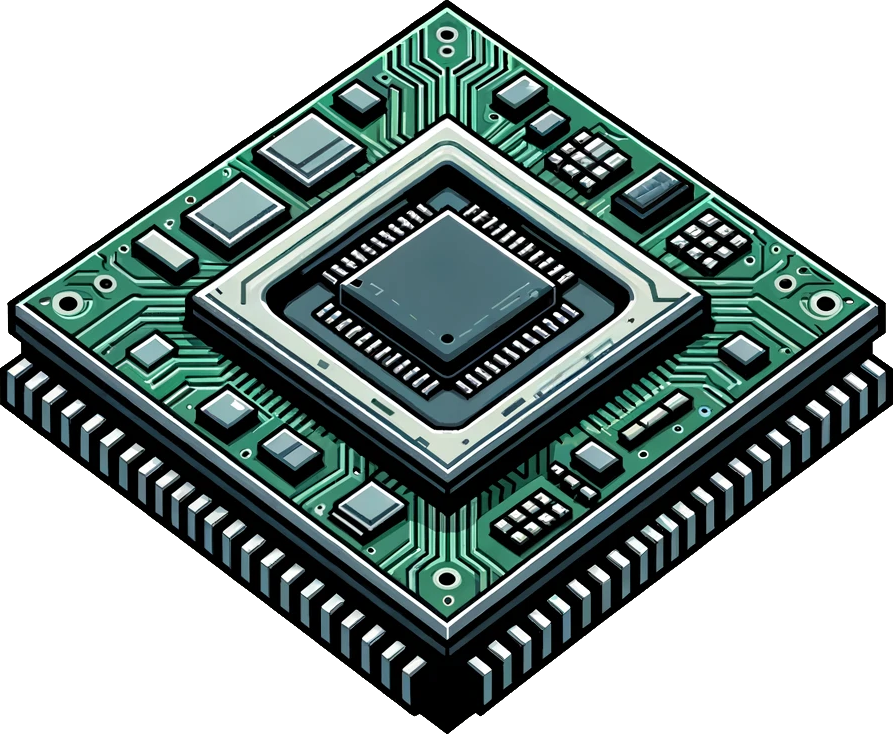
\includegraphics[scale=0.065]{images/cpu}};
}
\node at ($(first-cpu.east) + (-13pt, 6pt)$) {
  \begin{minipage}{1.5cm}
    \largeIcon{first.test, second.test, third.test}
  \end{minipage}%
};
\node[below=.3ex] at (first-cpu.south) { used };
\node[below=.3ex] at (second-cpu.south) { unused };
\node[below=.3ex] at (third-cpu.south) { unused };
\end{tikzpicture}%